\documentclass{beamer}
\usetheme{Madrid}
\usecolortheme{default}
\usepackage{listings}
\usepackage{tcolorbox}
\tcbuselibrary{listings, skins}

\newtcblisting{mycode}{
  arc=0mm,                          % Sharp corners
  boxrule=0.5pt,                    % Border thickness
  colback=white,                    % Background color
  colframe=black,                   % Border color
  listing only, 
  listing options={
    language=Python,
    basicstyle=\small\ttfamily,      % Monospace font
    keywordstyle=\color{blue},       % Color for 'import', etc.
    commentstyle=\color{blue},       % Color for comments
    stringstyle=\color{red},
    showstringspaces=false,
    breaklines=true
  },
  sharp corners,
  enhanced,
}

\title{Discrete-1.2.27}
\author{INDHIRESH S-EE25BTECH11027}
\date{\today}

\begin{document}

\begin{frame}
    \titlepage
\end{frame}

\begin{frame}{Question}
The polynomial p(x) = $x^5 + x^2 + 2$ has 
\begin{columns}[t]
    \begin{column}{0.45\textwidth}
        \begin{enumerate}[a)]
            \item all real roots
            \item 3 real and 2 complex roots
        \end{enumerate}
    \end{column}
    
    \begin{column}{0.45\textwidth}
        \begin{enumerate}[a)]
            \setcounter{enumi}{2} % Starts the count at 'c'
            \item 1 real and 4 complex roots
            \item all complex roots
        \end{enumerate}
    \end{column}
\end{columns}
\end{frame}



\begin{frame}{The Challenge}
    We need to find how many real and complex roots the polynomial $p(x) = x^5 + x^2 + 2$ has.
    \begin{itemize}
        \item Degree = 5 $\rightarrow$ Total of \textbf{5 roots}.
        \item Strategy: Use Descartes' Rule of Signs to narrow down the possibilities.
    \end{itemize}
\end{frame}

\begin{frame}{Explaining Descartes' Rule of Signs}
    This rule relates the number of \textbf{sign changes} in a polynomial's coefficients to the number of its real roots.
    
    \begin{block}{The Two-Step Process}
    \begin{enumerate}
        \item \textbf{Positive Roots:} Count sign changes in $p(x)$.
        \item \textbf{Negative Roots:} Count sign changes in $p(-x)$.
    \end{enumerate}
    \end{block}
    \textit{Note: The actual number of roots is either equal to the count of sign changes or less than it by an even integer.}
\end{frame}


\begin{frame}{ Positive Real Roots}
    Write out $p(x)$ and look at the signs of the coefficients:
    $$p(x) = \underbrace{+}_{\text{Term 1}} x^5 \quad \underbrace{+}_{\text{Term 2}} x^2 \quad \underbrace{+}_{\text{Term 3}} 2$$
    
    \begin{itemize}
        \item Sign sequence: $(+, +, +)$
        \item \textbf{Number of sign changes: 0}
    \end{itemize}
    
    \begin{alertblock}{Conclusion for Positive Roots}
        There are \textbf{zero} positive real roots. The graph will never touch the x-axis to the right of the y-axis.
    \end{alertblock}
\end{frame}

\begin{frame}{Negative Real Roots}
    Substitute $(-x)$ into the equation:
    $$p(-x) = (-x)^5 + (-x)^2 + 2$$
    $$p(-x) = \underbrace{-}_{\text{Term 1}} x^5 \quad \underbrace{+}_{\text{Term 2}} x^2 \quad \underbrace{+}_{\text{Term 3}} 2$$
    
    \begin{itemize}
        \item Sign sequence: $(-, +, +)$
        \item \textbf{Number of sign changes: 1} (from $-x^5$ to $+x^2$)
    \end{itemize}
    
    \begin{alertblock}{Conclusion for Negative Roots}
        There is exactly \textbf{1 negative real root}.
    \end{alertblock}
\end{frame}


\begin{frame}{ Finding Critical Points(Cross check)}
    To find where the graph "turns," we take the first derivative:
    $$p'(x) = 5x^4 + 2x$$
    Set $p'(x) = 0$:
    $$x(5x^3 + 2) = 0$$
    
    \textbf{Critical Points:}
    \begin{itemize}
        \item $x_1 = 0$
        \item $x_2 = \sqrt[3]{-0.4} \approx -0.74$
    \end{itemize}
\end{frame}


\begin{frame}{ The Second Derivative Test}
    We use $p''(x)$ to confirm the nature of these points:
    $$p''(x) = 20x^3 + 2$$
    
    \begin{block}{Testing $x = 0$ (Local Minimum)}
        $p''(0) = 2 > 0$ (Concave Up). \\
        Value: $p(0) = \mathbf{2}$
    \end{block}
    
    \begin{block}{Testing $x \approx -0.74$ (Local Maximum)}
        $p''(-0.74) = -6 < 0$ (Concave Down). \\
        Value: $p(-0.74) \approx \mathbf{2.32}$
    \end{block}
\end{frame}
\begin{frame}{ End Behavior \& Existence of Roots}
    We examine the limits of $p(x) = x^5 + x^2 + 2$ as $x$ grows large:
    
    \begin{itemize}
        \item As $x \to \infty$, $p(x) \approx x^5 \to \infty$
        \item As $x \to -\infty$, $p(x) \approx x^5 \to -\infty$
    \end{itemize}

    \begin{block}{Intermediate Value Theorem (IVT)}
        Since $p(x)$ is a continuous polynomial that changes sign from negative to positive over its domain, there must be \textbf{at least one} value $c$ such that $p(c) = 0$.
    \end{block}
    
    \textbf{Conclusion:} This confirms the existence of at least \textbf{one real root}.
\end{frame}
\begin{frame}{Putting it all together}
    \begin{itemize}
        \item The lowest point of the "wiggle" is $y = 2$ (at $x=0$).
        \item Since the local minimum is \textbf{above the x-axis}, the graph never crosses back down.
        \item The only time $p(x)$ is negative is when $x < -1.29$.
    \end{itemize}
    
    \begin{center}
        \textbf{Conclusion:} 1 real crossing, 4 hidden (complex) roots.
    \end{center}
\end{frame}
\begin{frame}[fragile]
\frametitle{Python Code for Plot}

\begin{mycode}
import matplotlib.pyplot as plt
import numpy as np

# Define the polynomial function
def p(x):
    return x**5 + x**2 + 2

# Create an array of x values
x = np.linspace(-1.5, 1, 400)
y = p(x)

# Create the plot
plt.figure(figsize=(10, 6))
plt.plot(x, y, label='$p(x) = x^5 + x^2 + 2$', color='blue', linewidth=2)


\end{mycode}

\end{frame}

\begin{frame}[fragile]
\frametitle{Python Code for Plot}

\begin{mycode}
# Add x and y axis lines
plt.axhline(0, color='black', linewidth=1)
plt.axvline(0, color='black', linewidth=1)


from scipy.optimize import fsolve
real_root = fsolve(p, -1)[0]
plt.plot(real_root, 0, 'ro', label=f'Real Root $\\approx {real_root:.3f}$')

tp1_x = 0
tp1_y = p(tp1_x)
tp2_x = (-0.4)**(1/3) if (-0.4) >= 0 else -abs(-0.4)**(1/3)
tp2_y = p(tp2_x)



\end{mycode}

\end{frame}

\begin{frame}[fragile]
\frametitle{Python Code for Plot}

\begin{mycode}
plt.plot(tp1_x, tp1_y, 'go', label=f'Local Min (0, {tp1_y})')
plt.plot(tp2_x, tp2_y, 'mo', label=f'Local Max ({tp2_x:.2f}, {tp2_y:.2f})')

# Add labels and title
plt.title('Plot of $p(x) = x^5 + x^2 + 2$', fontsize=14)
plt.xlabel('x', fontsize=12)
plt.ylabel('p(x)', fontsize=12)
plt.grid(True, linestyle='--', alpha=0.7)
plt.legend()

plt . tight_layout ()
plt . show ()

\end{mycode}

\end{frame}
\begin{figure}
    \centering
    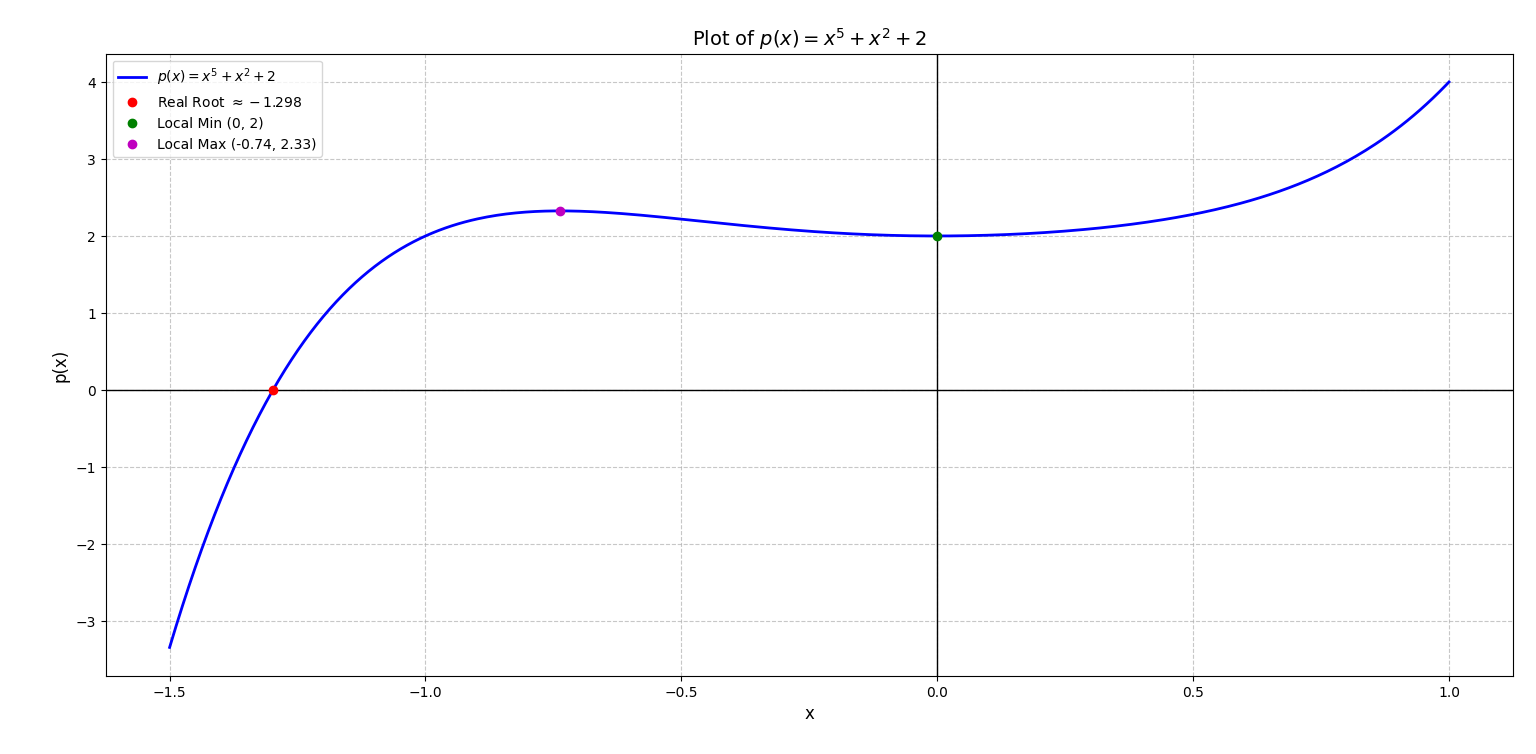
\includegraphics[width=\linewidth]{Plot.png}
    \caption{Python plot}
    \label{fig:placeholder}
\end{figure}
\end{document}